\graphicspath{{./Figs/}}

\chapter{Theory and Methodology}
This chapter outlines the theory and Methodology used create, test and collect the data required for the wing-propeller interaction analysis. 

\section{Material Choice}

\section{FreeCAD}
FreeCAD is a 3D parametric modeler and was used with provided python scripts to produce fuselage, wing and tail shapes when given input parameters to define the shape and geometry. Various model shapes were produced with the aim of making the model 3D printable in order to allow for ease of manufacturing and testing. Several design constraints had to be considered when developing the model due to the structural strength of the PLA used for 3D-printing and the limitations . the wings and tail could not be 
\todo{finish}

\section{VAP 3.5}
VAP 3.5 is a open-source software which uses the High-Order Free Wake (HOFW) \todo{abb} method in order to determine the aerodynamic performace of MAV designs. 


\section{Model Development}

\section{Wind Tunnel Testing}

\subsection{Wind Tunnel Setup}

The nano25 load cell was used to record the forces and moments acting on the model about the mounting position at 25\overline{c}. 

\begin{figure}[H]
    \centering
    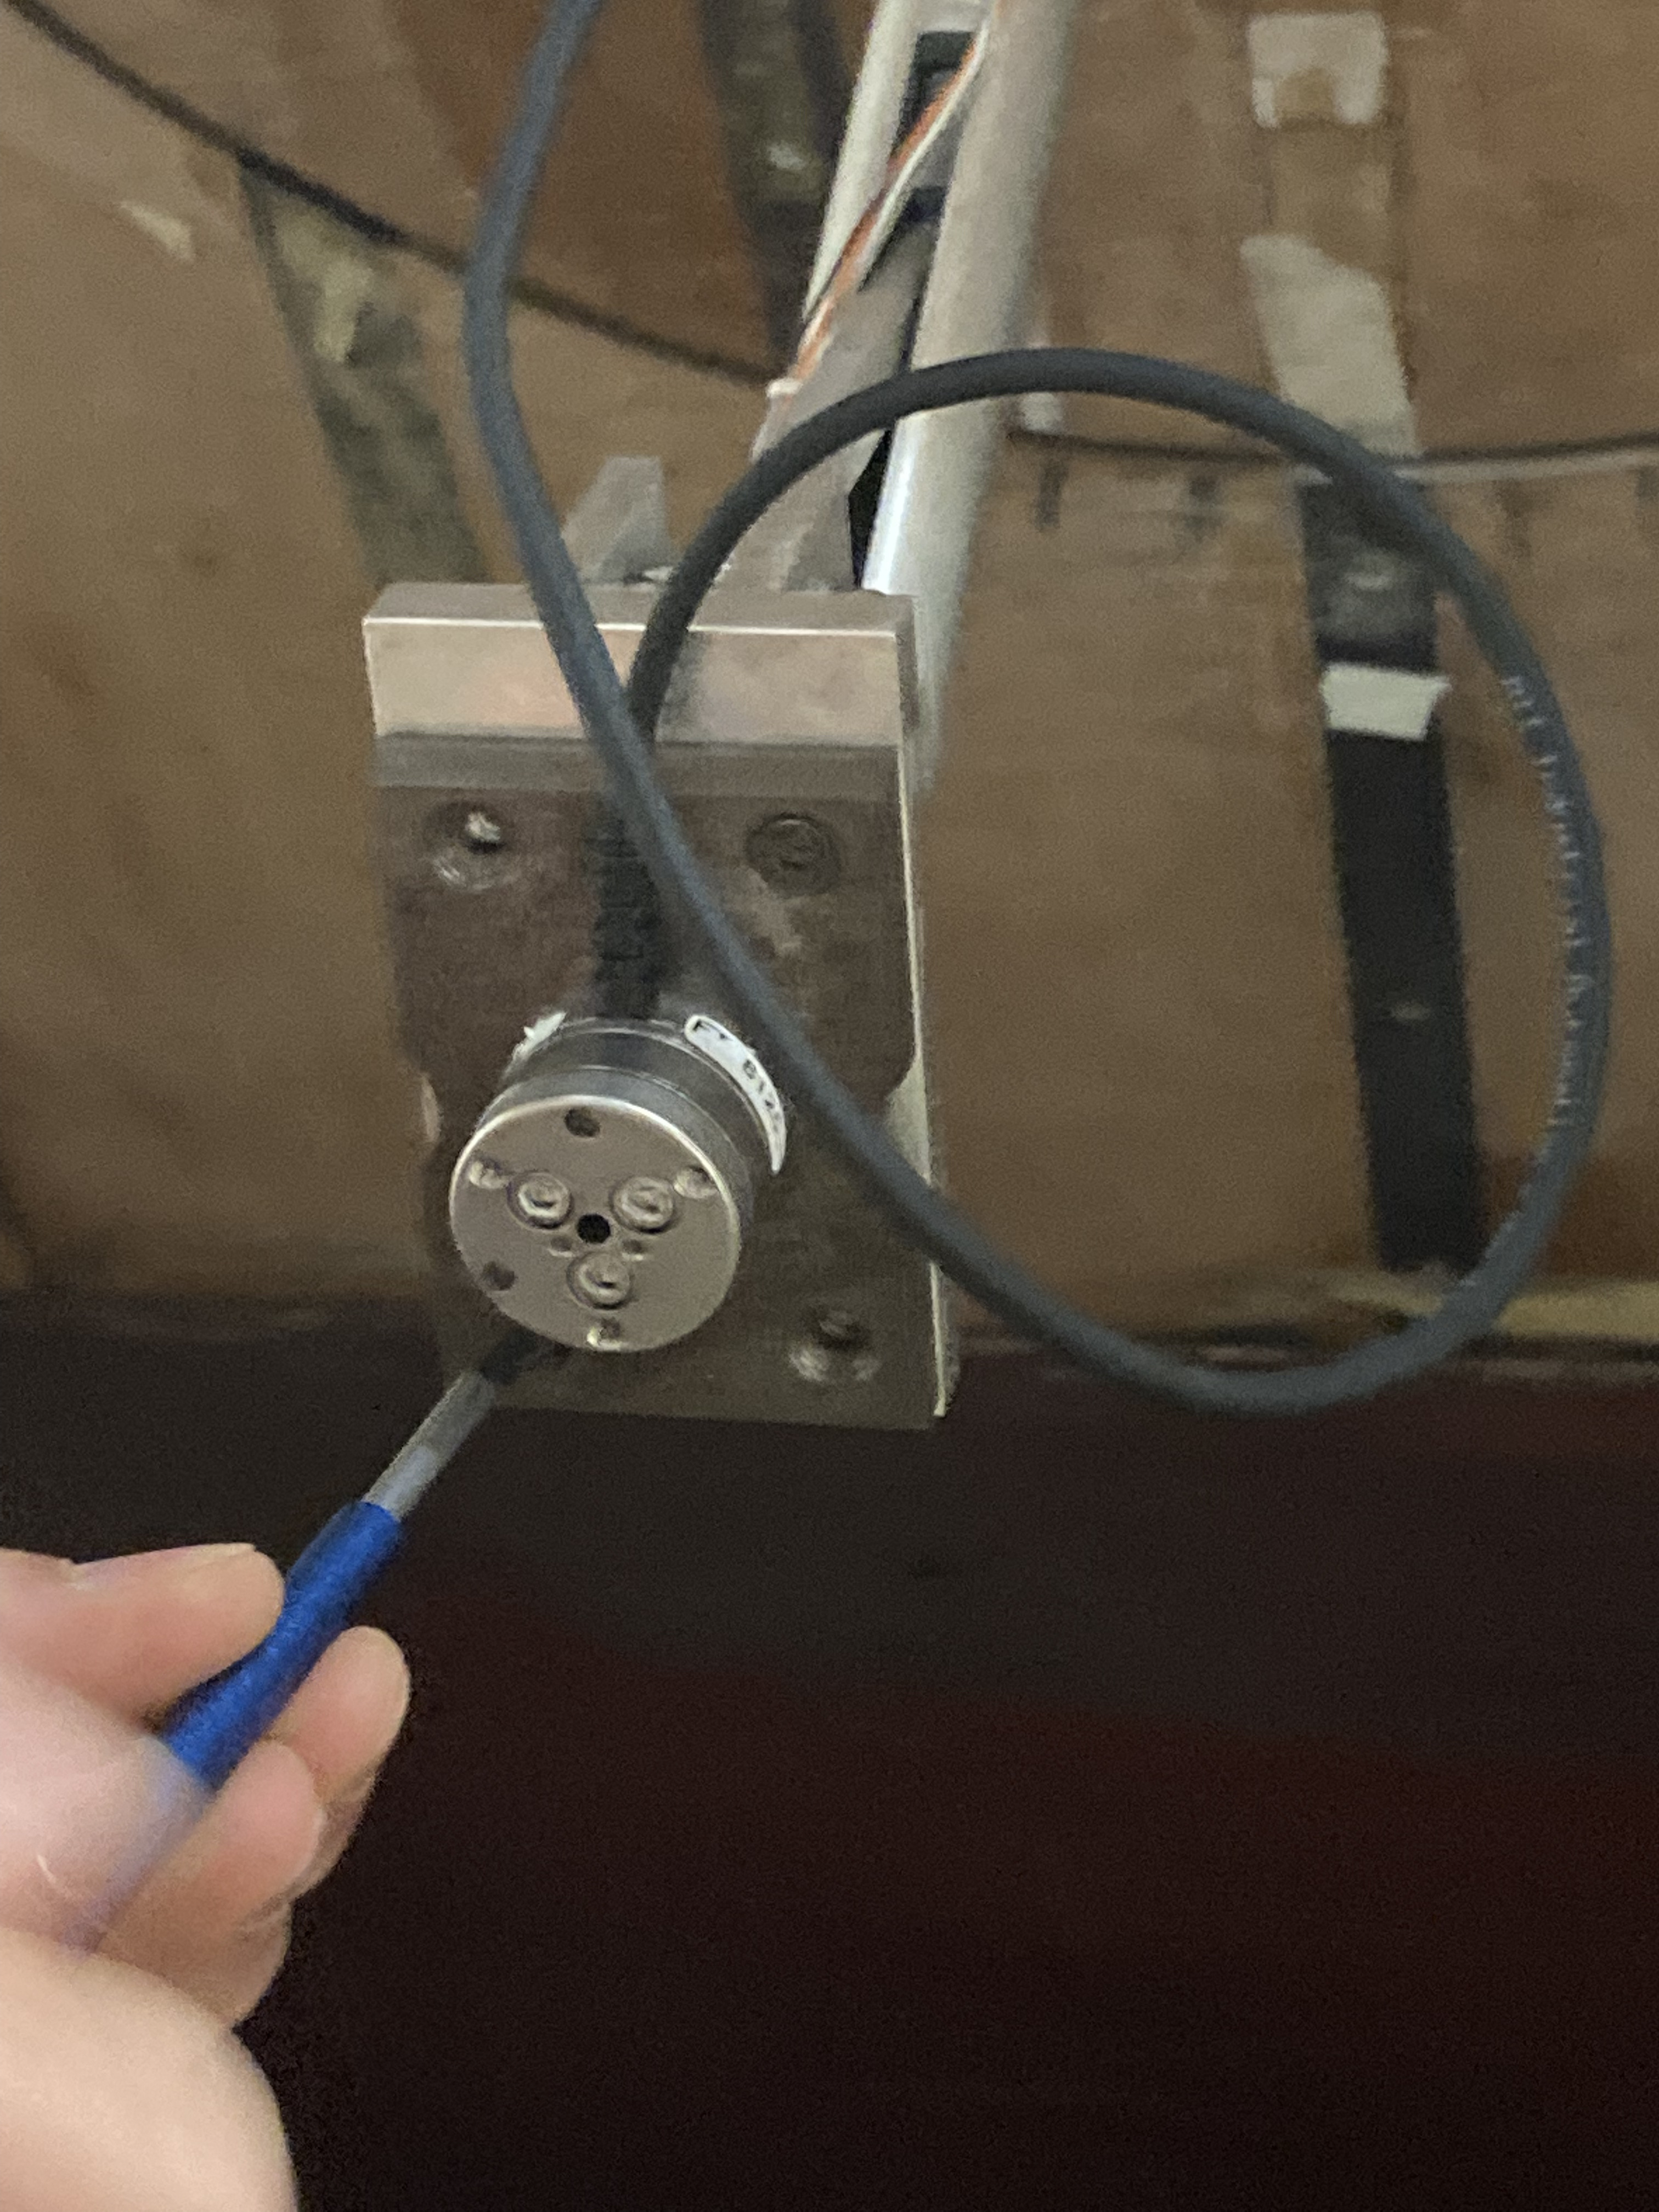
\includegraphics[scale=0.75]{04_Methodology/Figs/loadCellMount}
    \caption{Nano 25 load cell mount}
    \label{fig:LoadCella}
\end{figure}

The model mount was then attached over the load cell. 

\begin{figure}
    \centering
    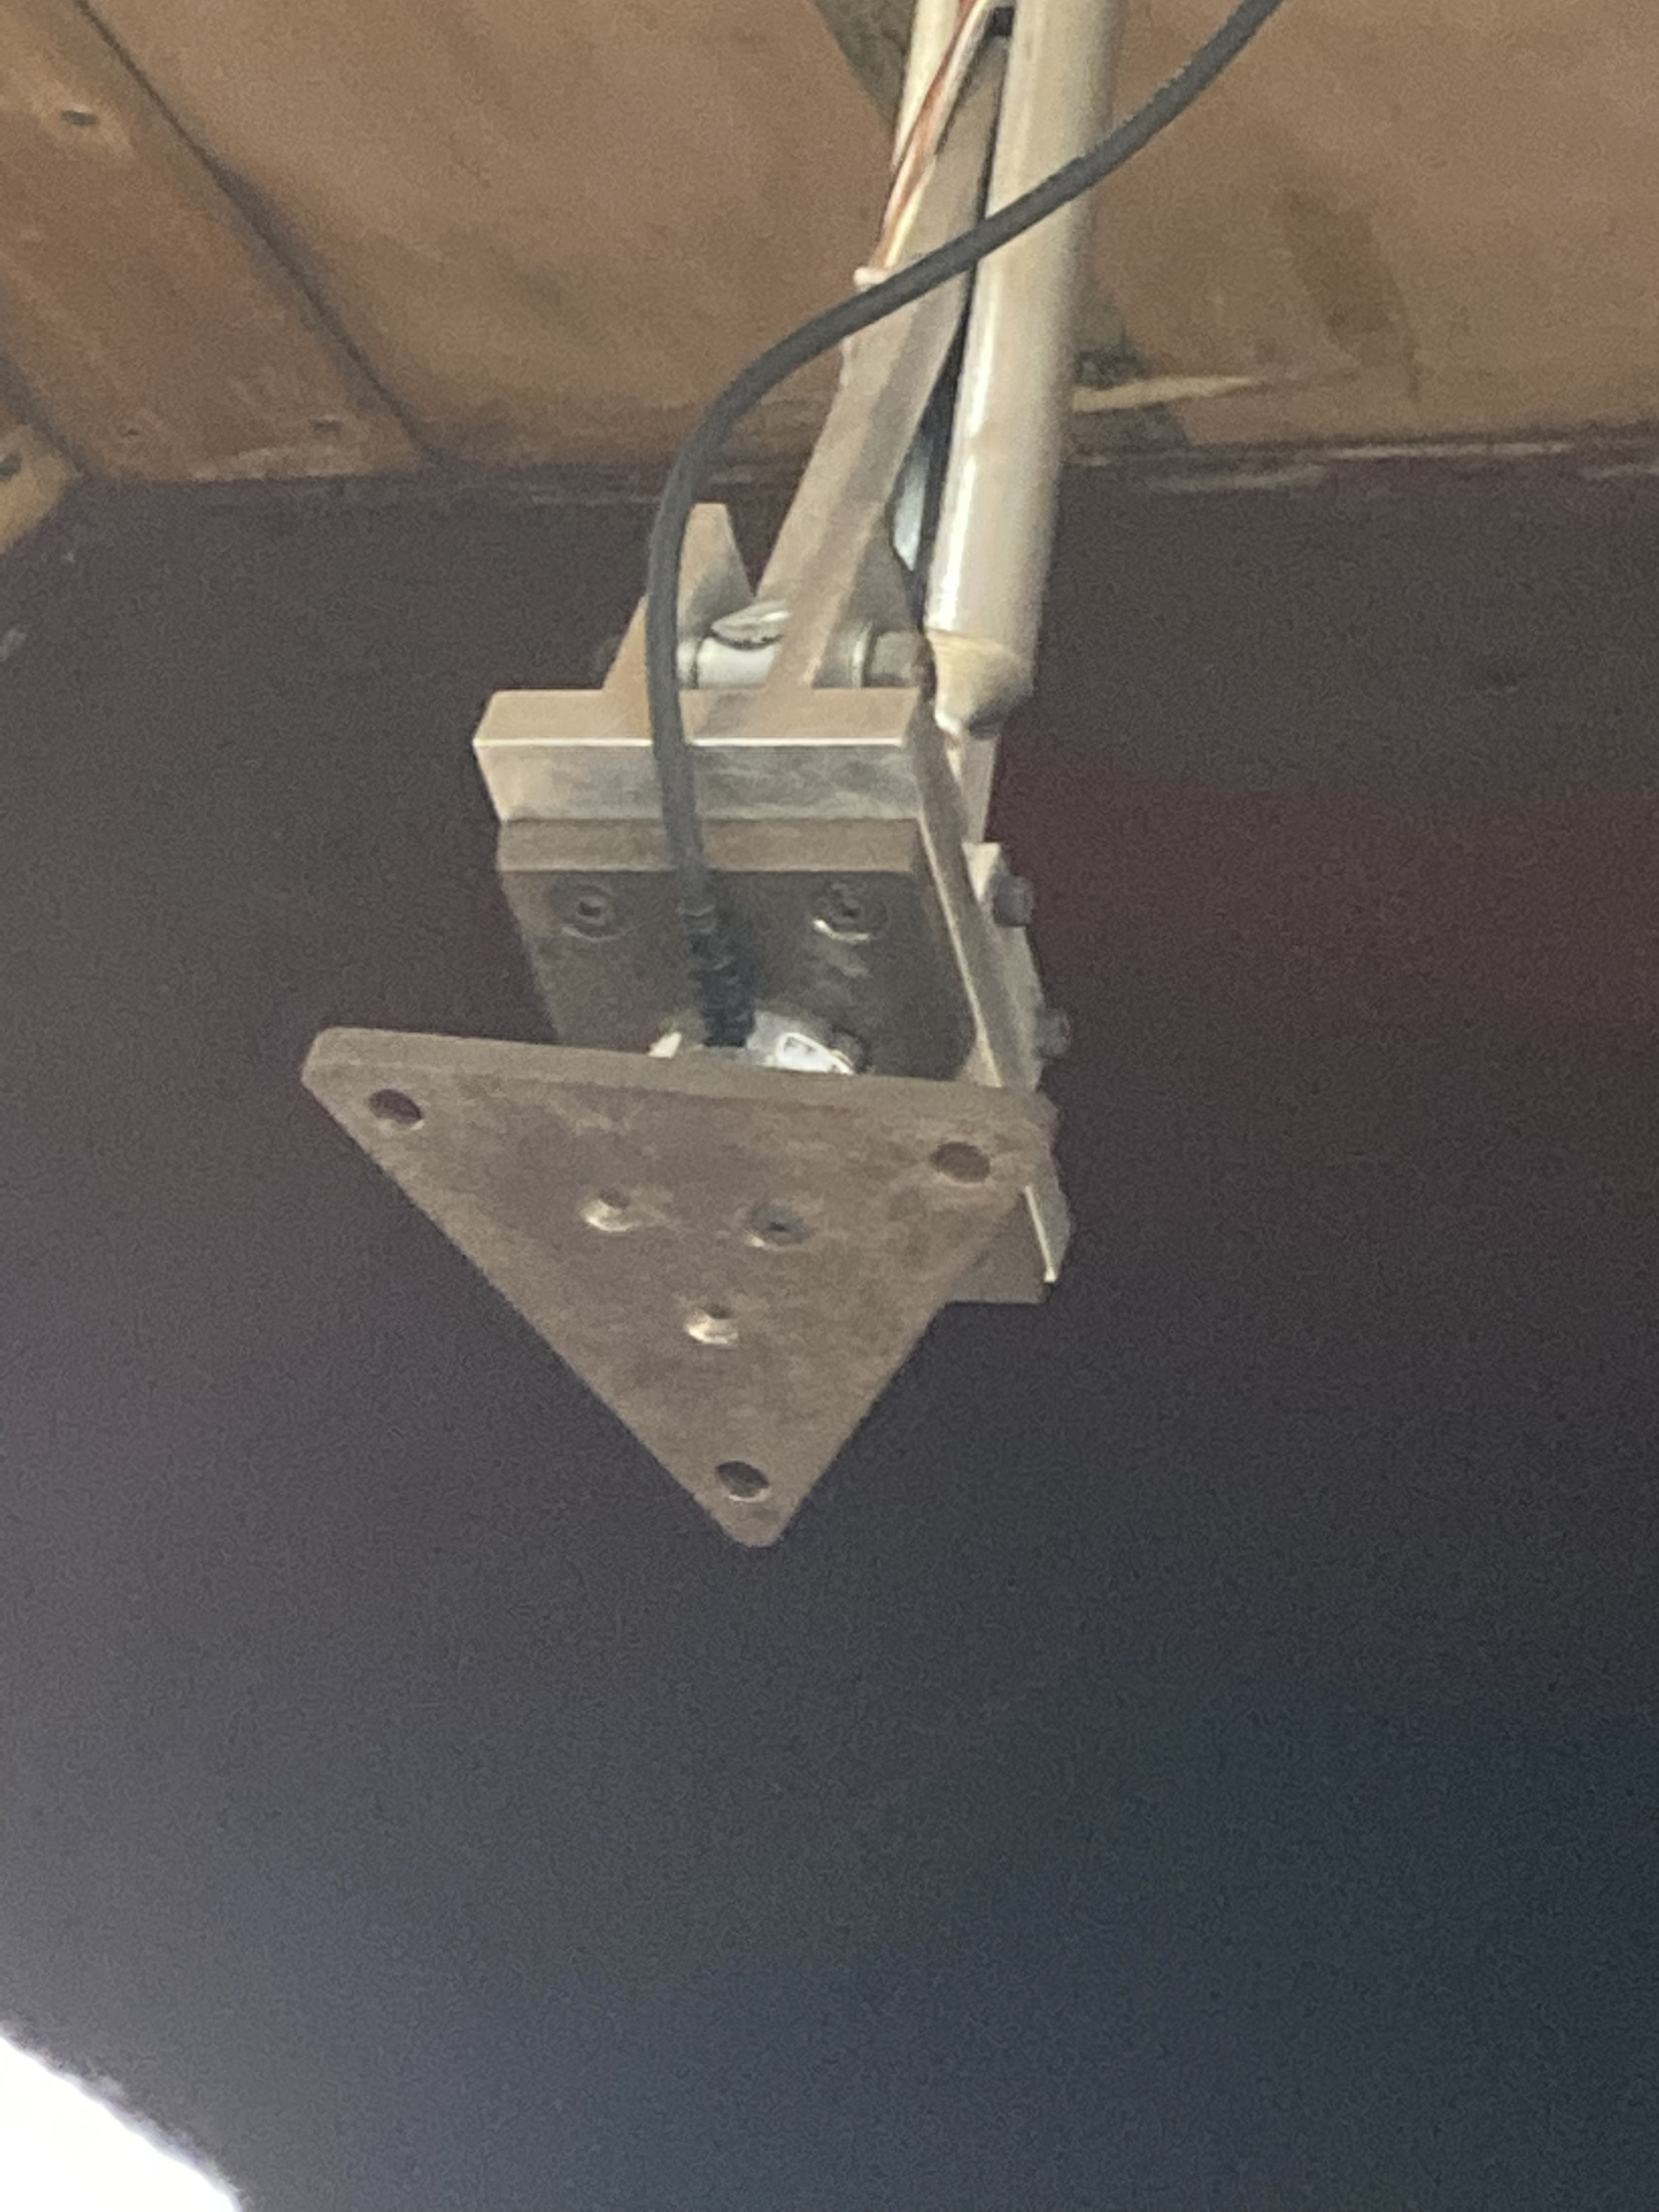
\includegraphics[scale=0.75]{04_Methodology/Figs/mount}
    \label{fig:LoadCellb}
\end{figure}

The model was then attached in three main configurations. These were mounting the propeller without a propeller, in a tractor and pusher configurations.

\begin{figure}
    \centering
    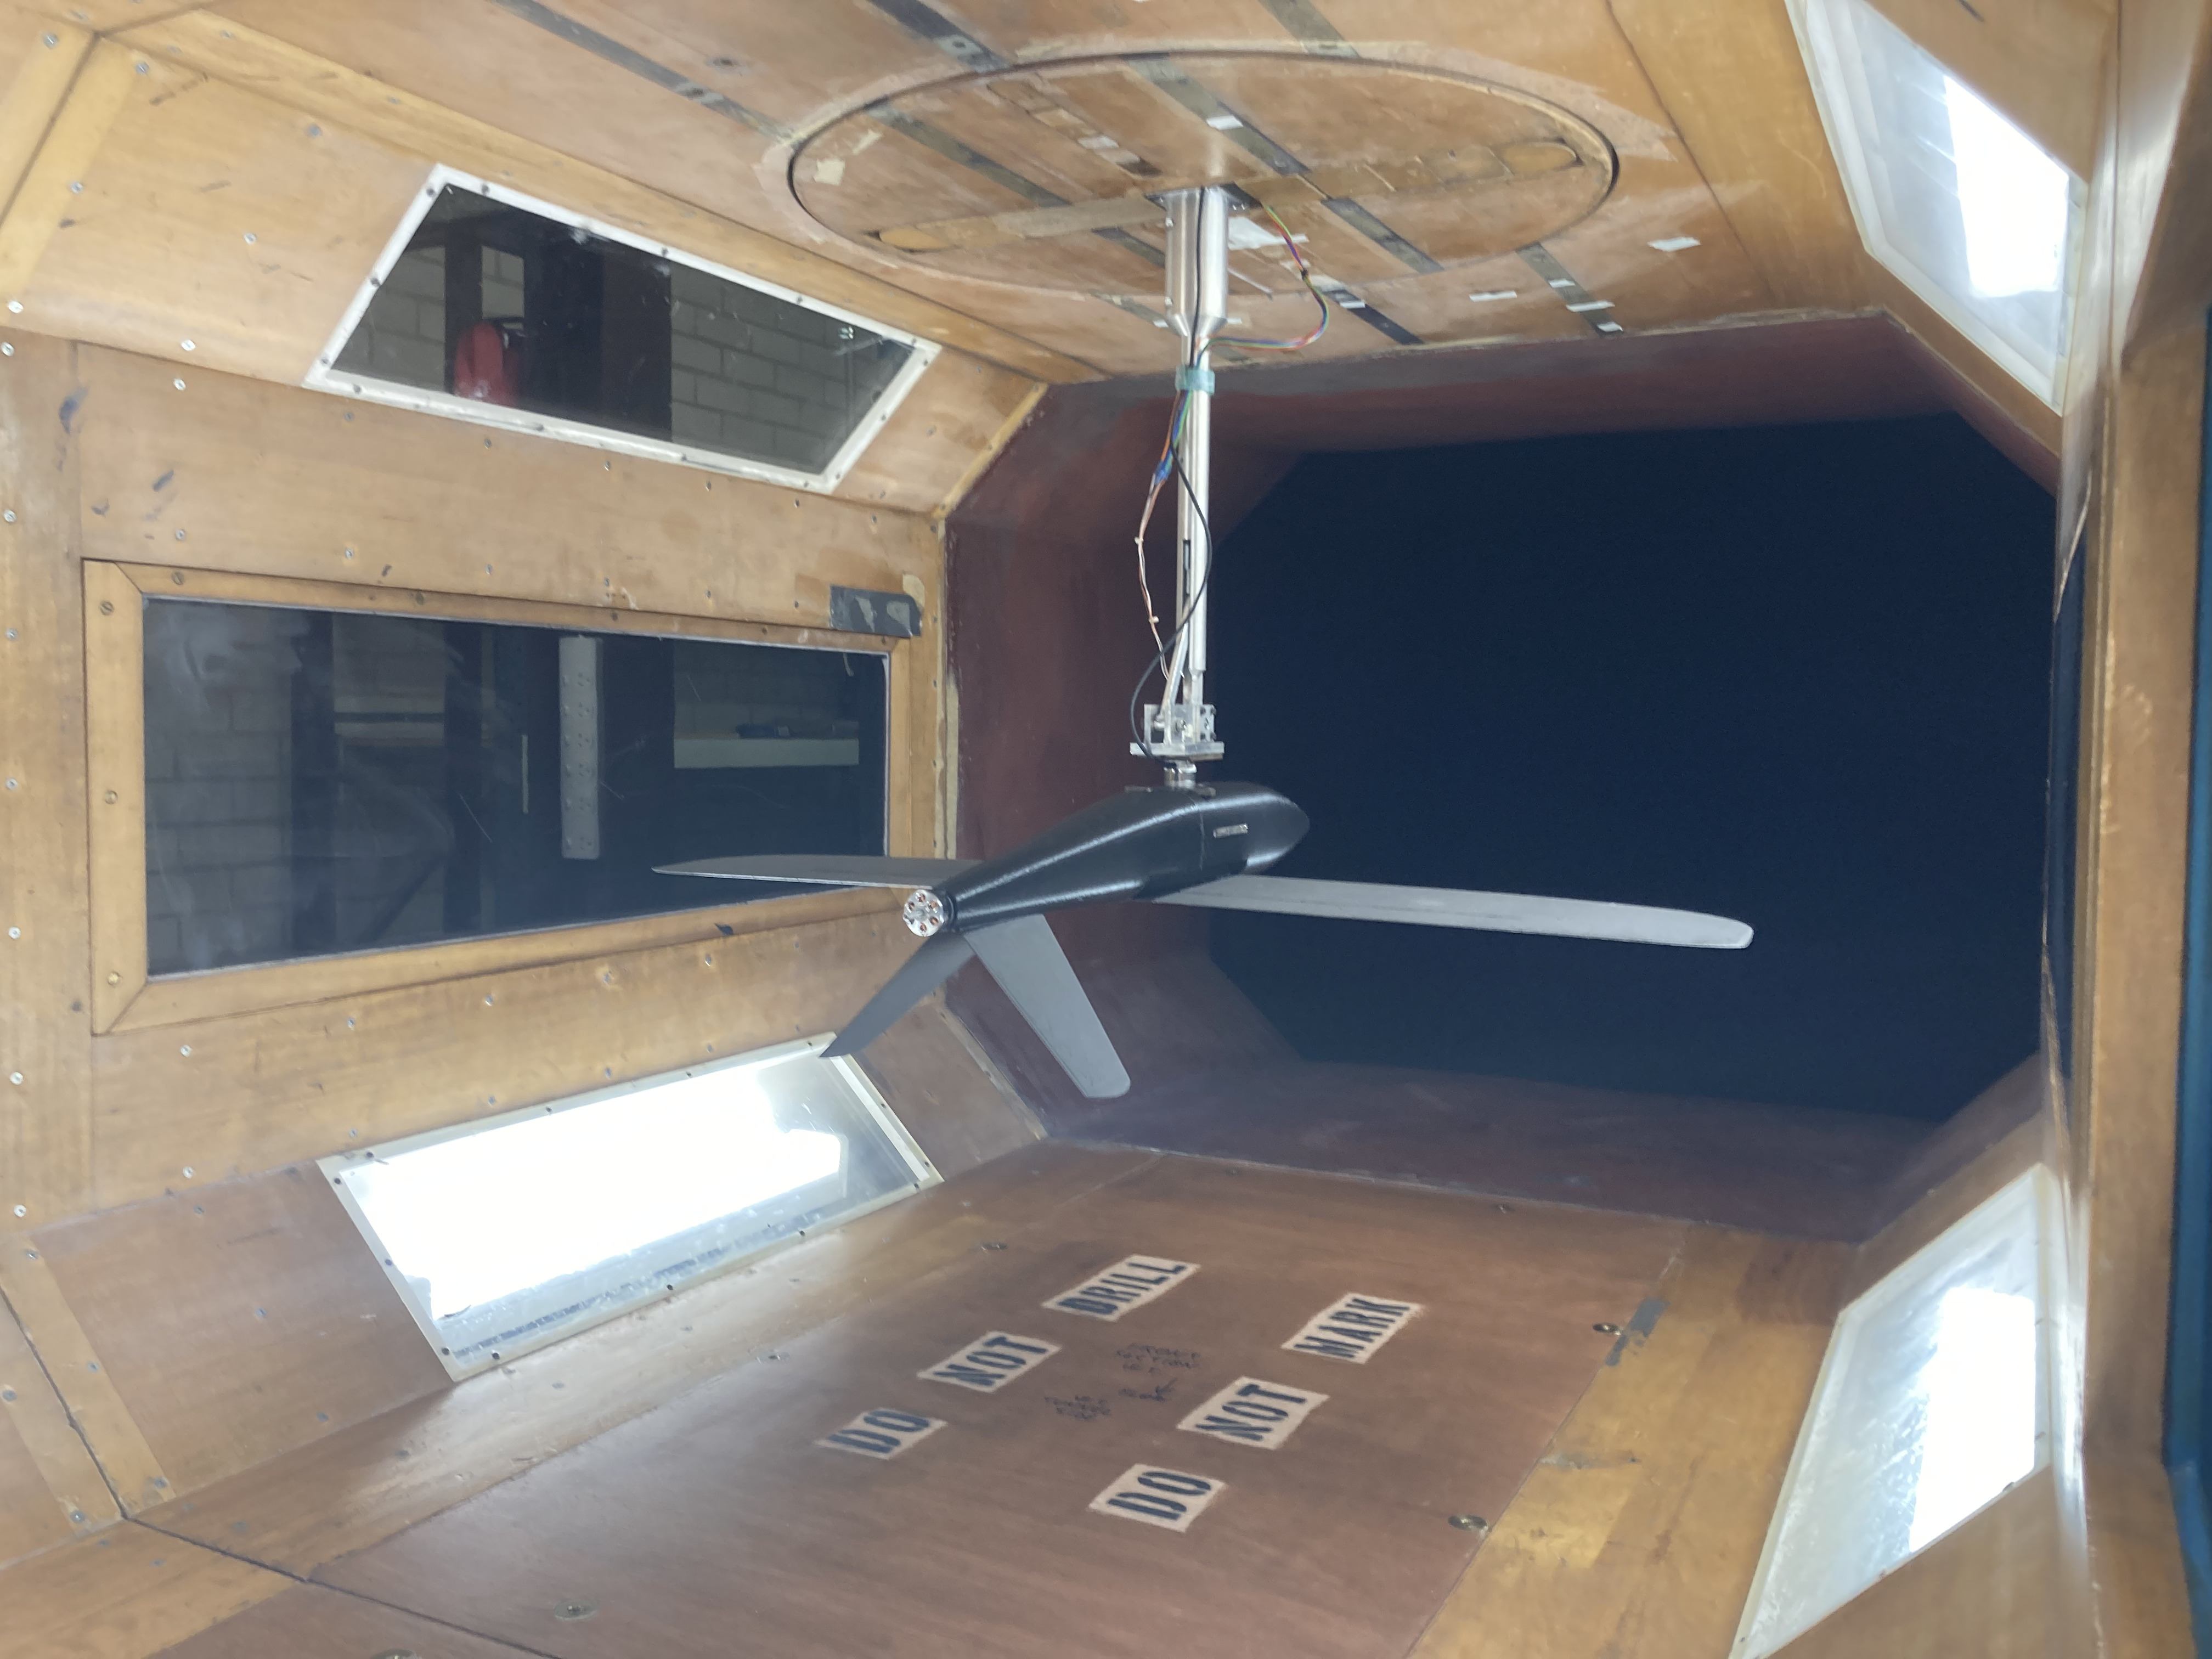
\includegraphics[]{04_Methodology/Figs/noprop}
    \label{fig:noprop}
\end{figure}

\begin{figure}
    \centering
    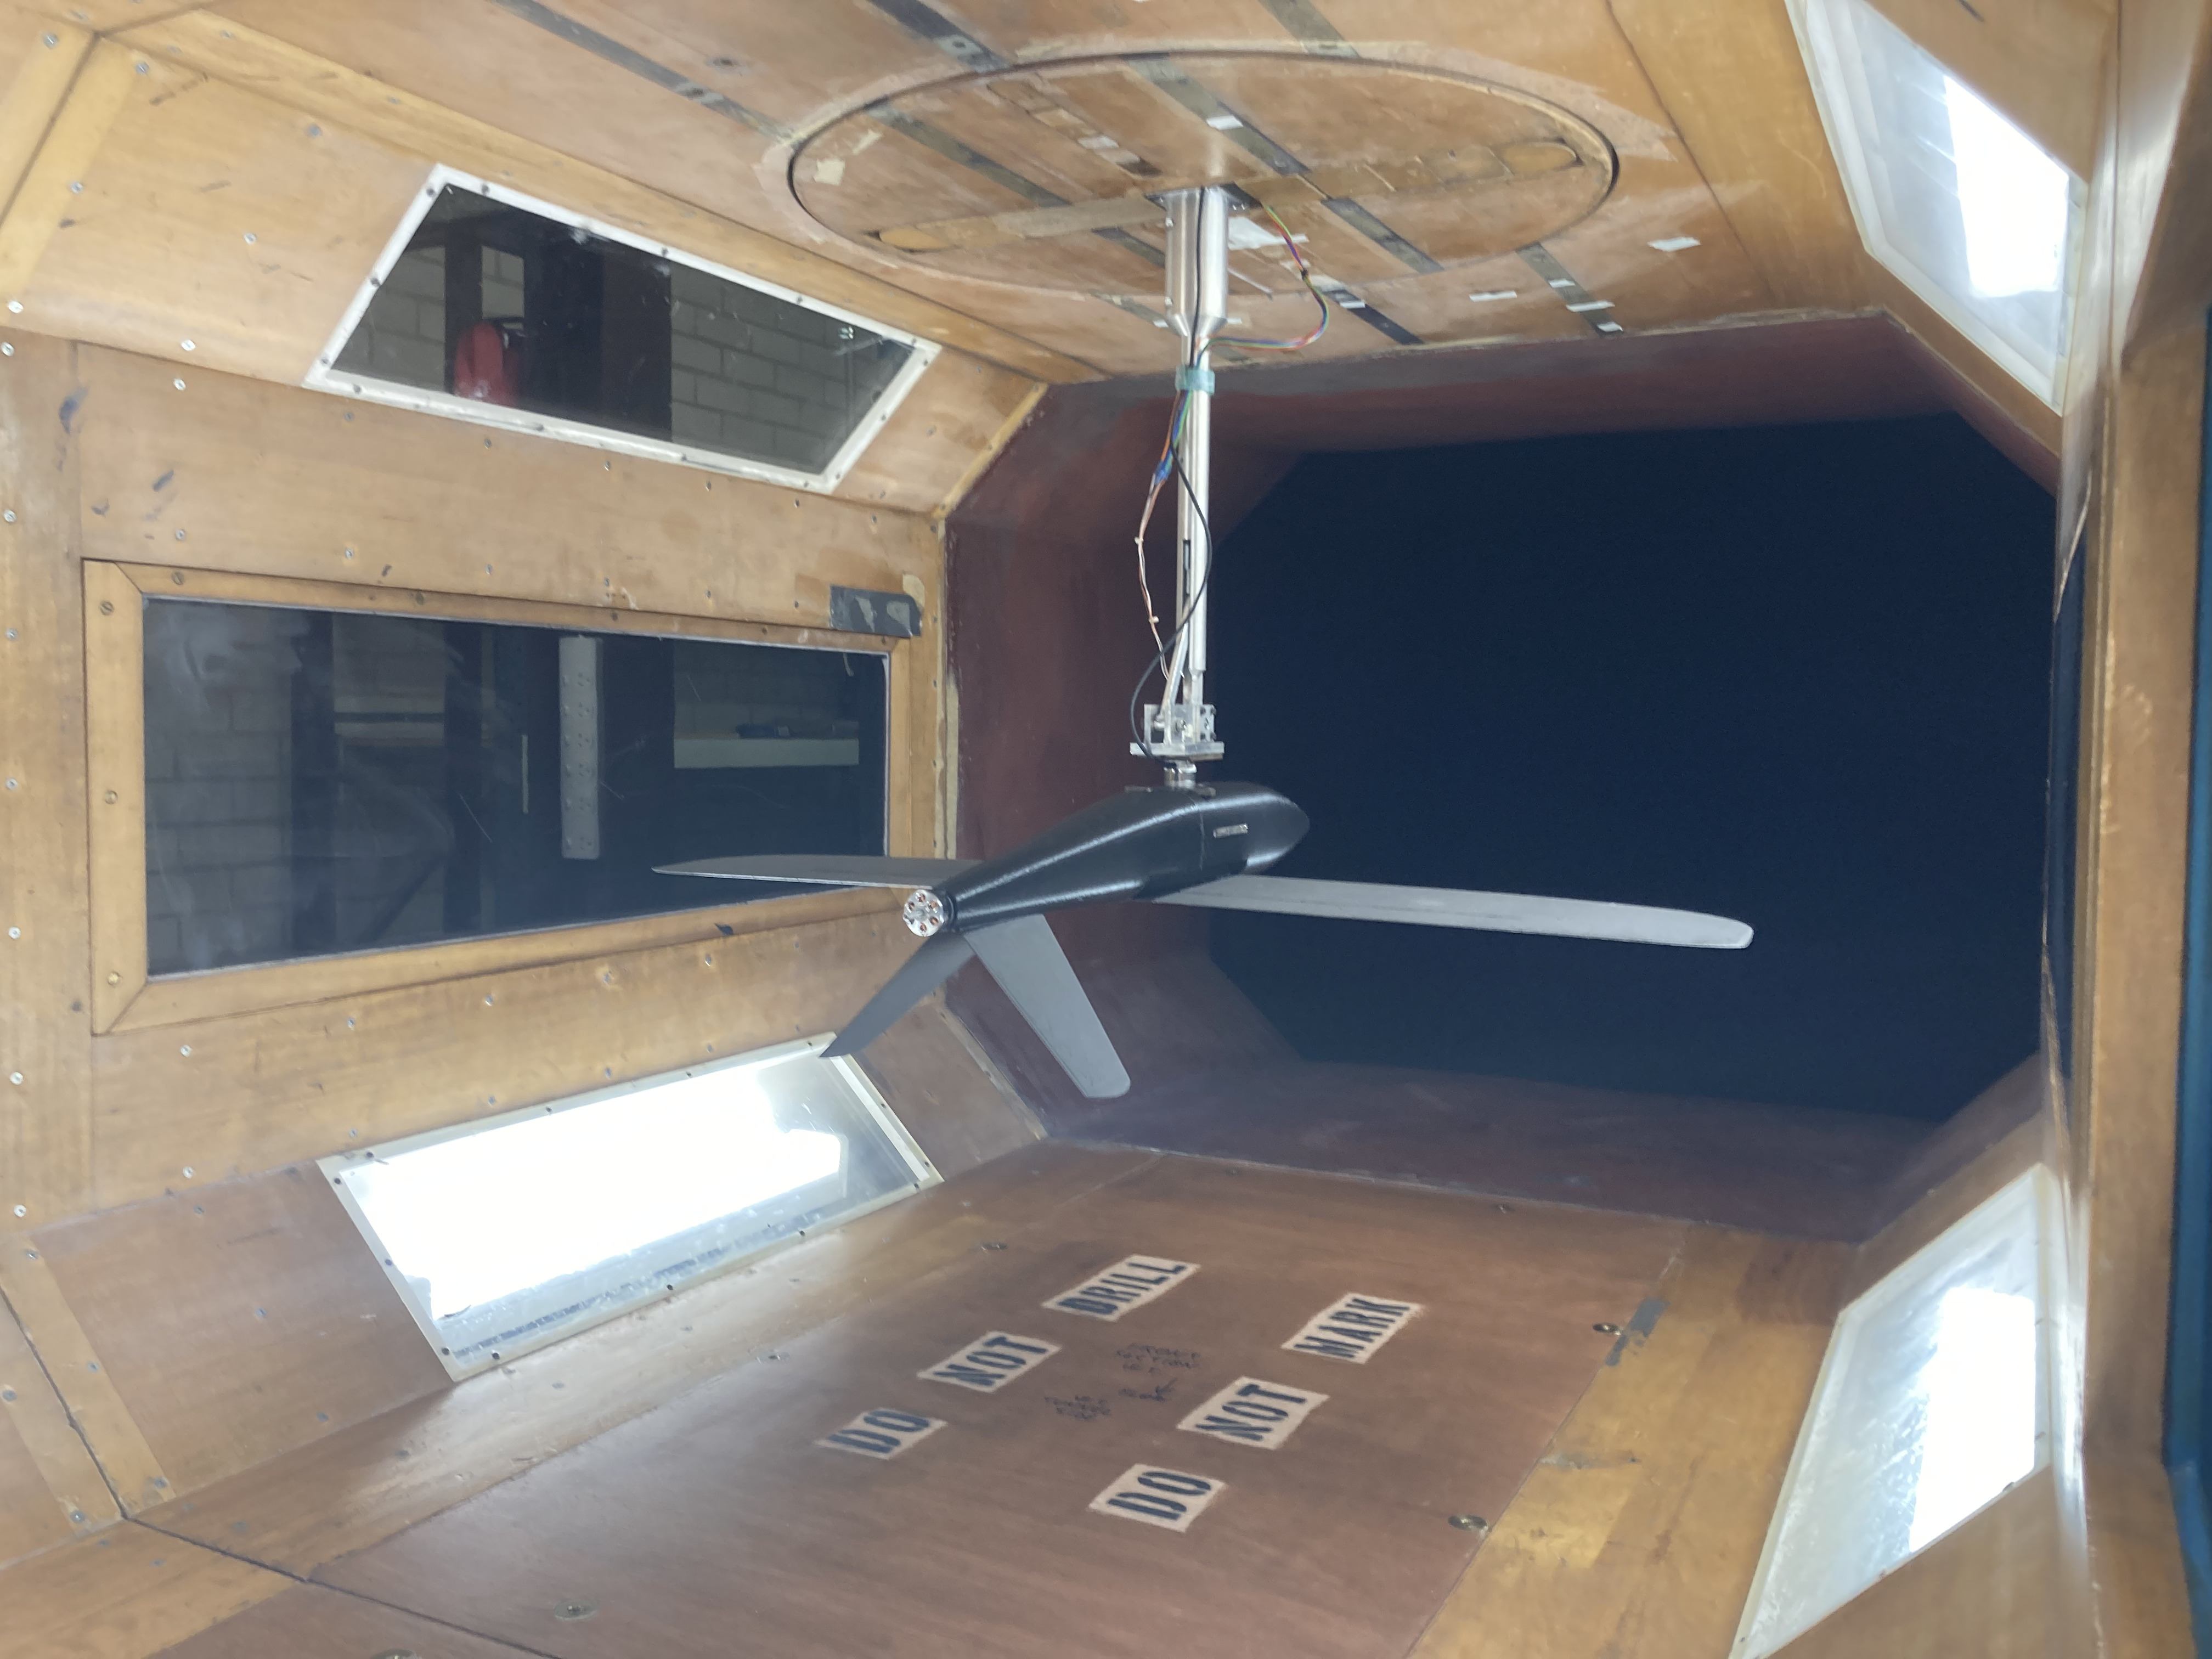
\includegraphics[]{04_Methodology/Figs/noprop}
    \label{fig:pusher}
\end{figure}


\begin{figure}
    \centering
    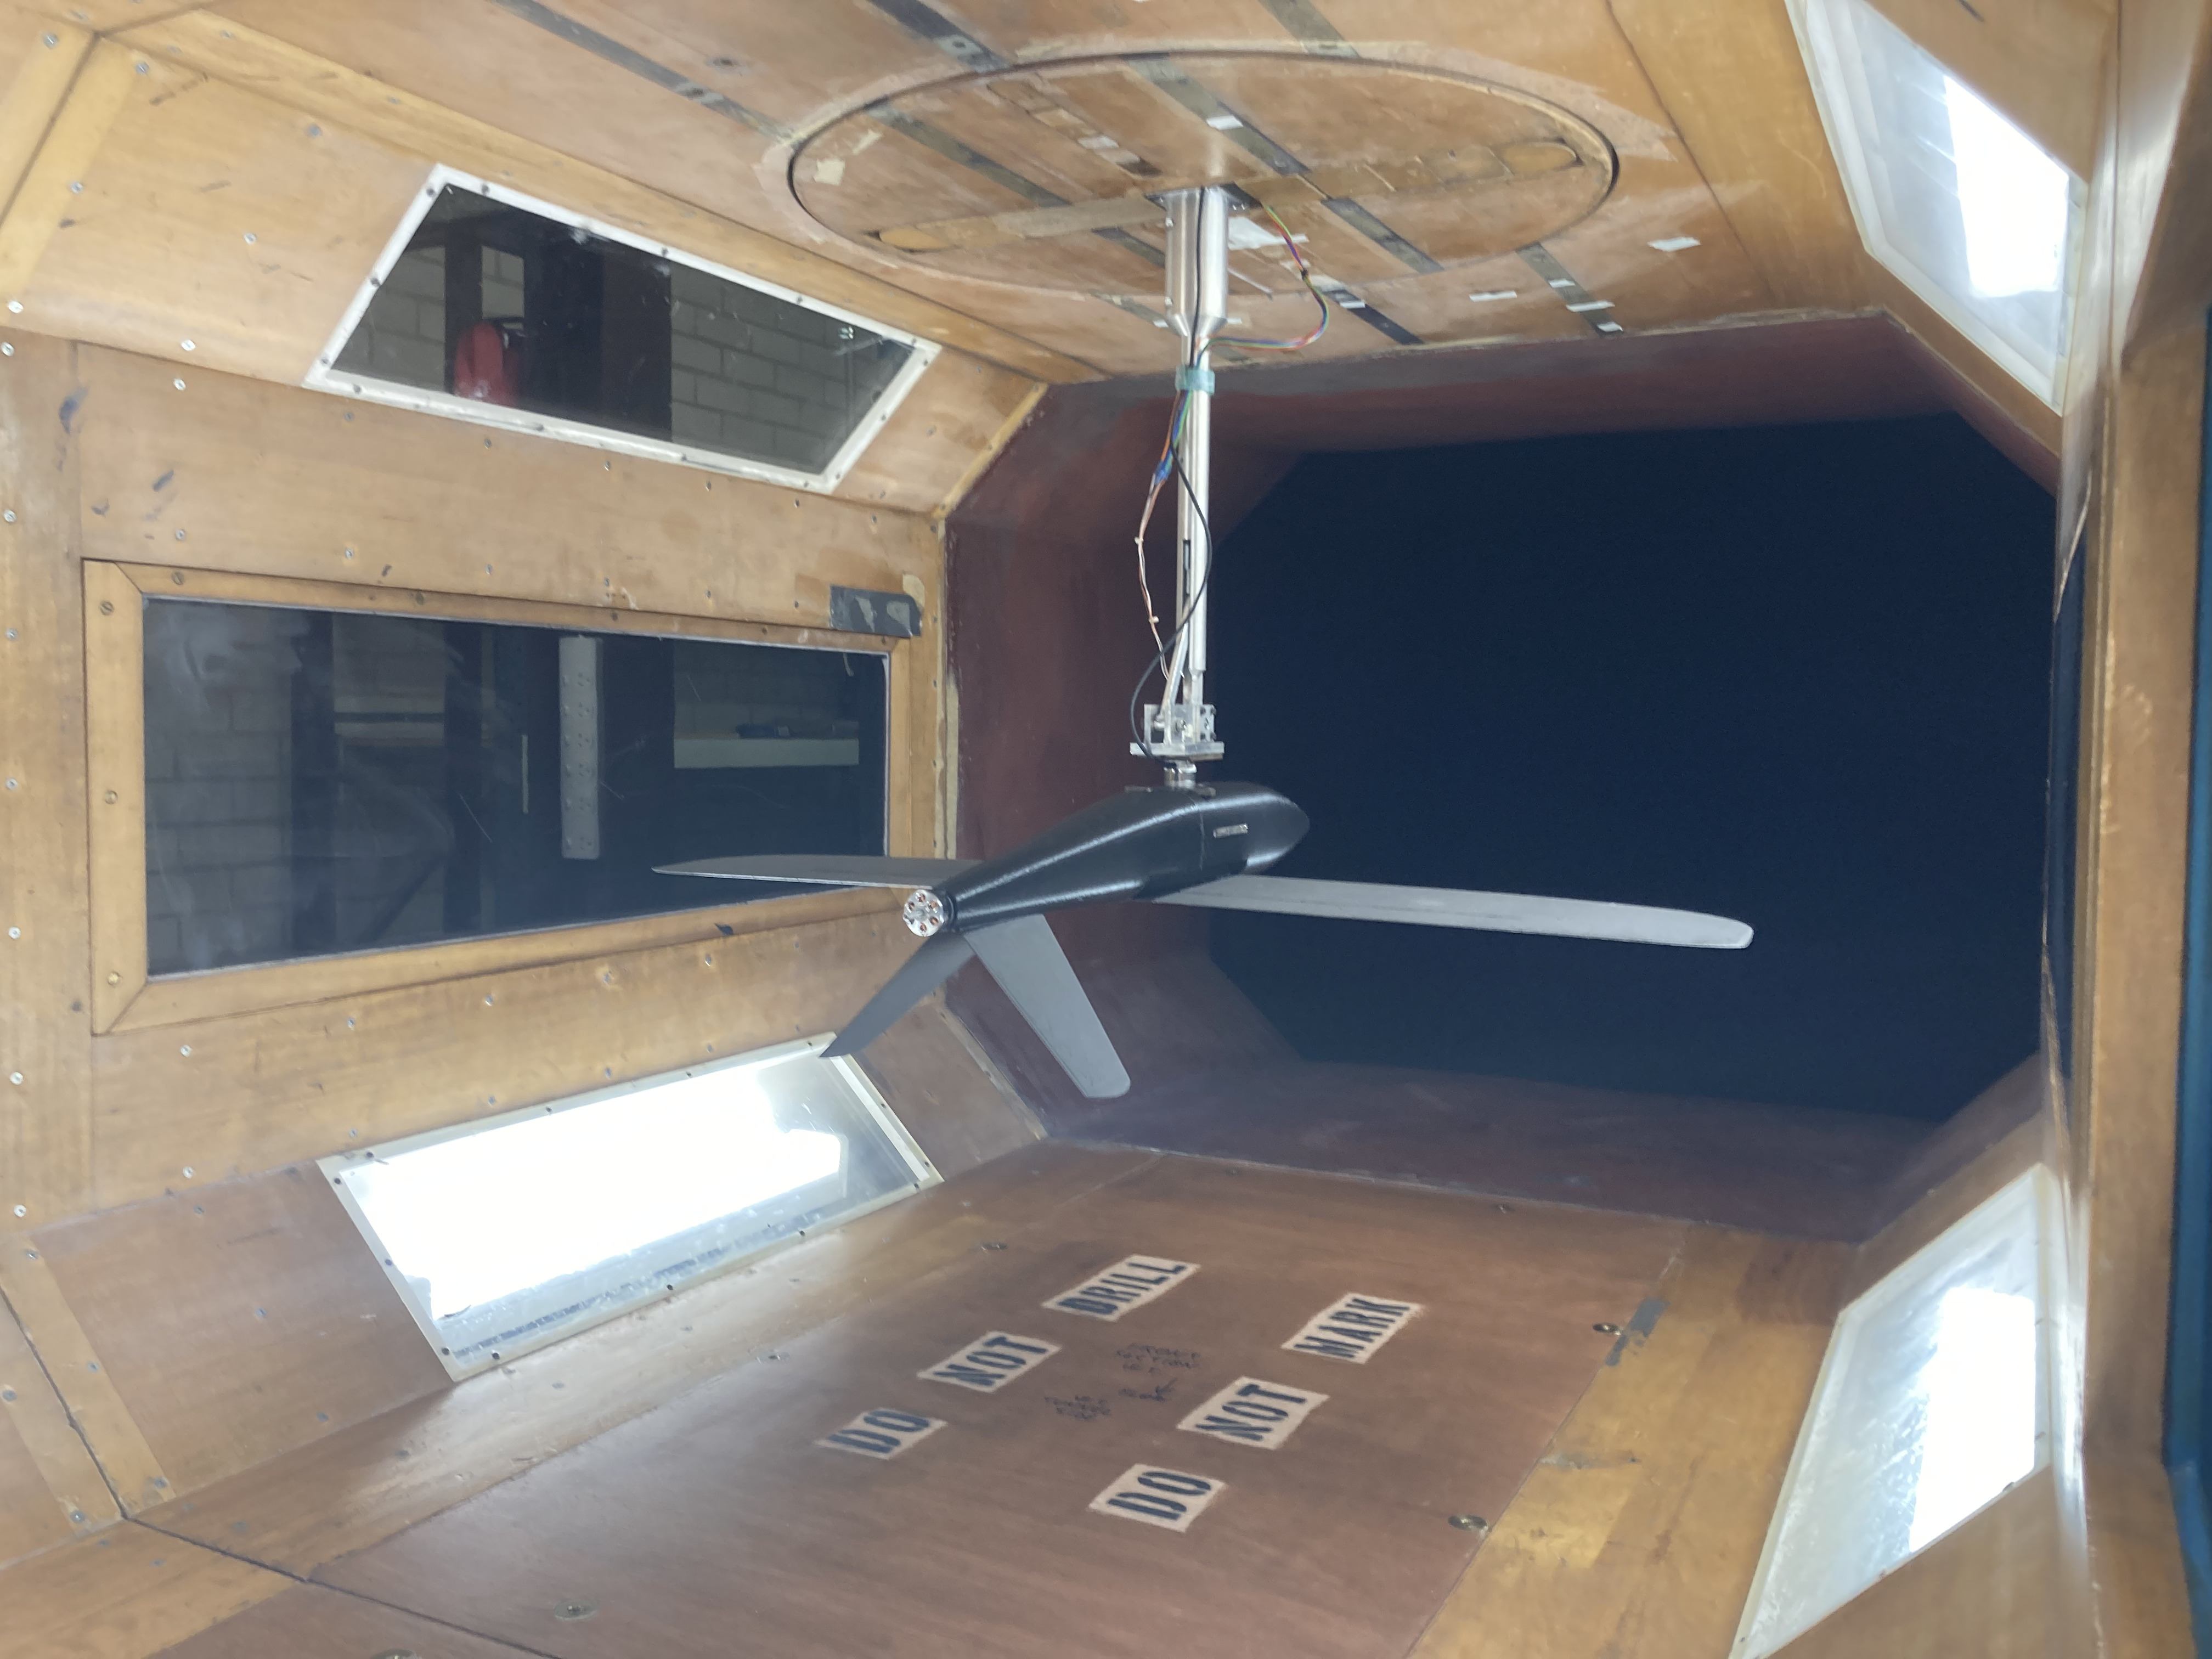
\includegraphics[]{04_Methodology/Figs/noprop}
    \label{fig:tractors}
\end{figure}



\section{Stability Calculation}
In order to determine the stability of the model in all the tested configurations the stability deratives of the model had to be determined. Data from the nano 25 load cell was used to determine the loads and moments acting on the model about the mounting point. These values were transformed \todo{right word?} to the neutral point of the model at 20\overline{c}. The aerodynamic coefficients were determined using equations \ref{eqn:lift} to \ref{eqn:drag} and the moment coefficients about the pitch, yaw and roll axis were calculated using Equations \ref{eqn:pitching} to \ref{eqn:yaw}. 





